% !TEX root = ../lectures_olympics.tex

\chapter{功和动能,机械能守恒}
\section{功,动能定理}

我们知道力是改变物体速度的原因,在外力的作用下物体的速度会发生变化。
之前学过的牛顿第二定律就是这一现象的集中表现,另外在第二定律的基础上我们还发展出了动量定理,它告诉我们力对时间的积累,也就是所谓的作用于物体的冲量会使该物体的动量发生变化。
除了动量还有一个物理量可以用来描写物体运动的性质,它称之为运动物体的动能,今天就来学习和它有关的物理。


\begin{figure}[htbp]
\begin{center}
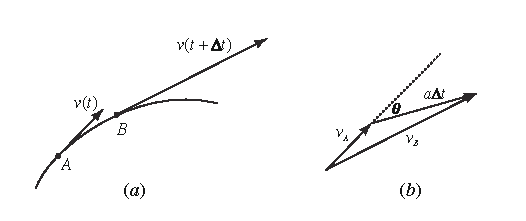
\includegraphics{images/energy-1.pdf}

\caption{在外力作用下的速度变化}
\label{fig: 动能定理:外力作用下的速度变化}
\end{center}
\end{figure}

如图\ref{fig: 动能定理:外力作用下的速度变化}所示,假设一个质量为$m$的物体有时刻$t$位于图中的$A$点,此时它的速度为$v(t)$,在外力作用下经过很小的$\Delta t$时间间隔到达了图中的$B$点,此时速度变为$v(t+\Delta t)$。
在曲线运动的讨论中我们知道对于极小的$\Delta t$物体在$B$点速度的大小,也就是速率$v_B$与在$A$点的速率$v_A$的差别由加速度的切线分量$a\cos\theta$所决定:
\begin{equation}
v_B^2 = v_A^2 + 2av_A\Delta t  \cos\theta
\end{equation}
进一步根据牛顿第二定律可以得到加速度和所受外力的关系为$a=F/m$,将它代入上式可得
\begin{equation}
v_B^2 = v_A^2 + 2\frac{F}{m}v_A\Delta t  \cos\theta
\end{equation}
右边最后一项当中的$v_A\Delta t$实际上就是在$\Delta t $时间里该物体运动位移的大小。
进一步整理就变成了
\begin{equation}\label{eqn: 动能定理}
F\Delta x\cos\theta = \frac{1}{2}mv_B^2-\frac{1}{2}mv_A^2.
\end{equation}

这就是动力学中的动能定理。
左边为力$F$与在力作用下的位移$\Delta x$以及力与位移的夹角$\theta$的余弦的乘积,也就是力在位移方向上的投影与位移的乘积,将它称之为力的\emph{功},因为上式是对一个小的时间间隔所给出的,此时功也是一个小量
\begin{equation}\label{eqn: 动能定理-功的微分}
\Delta W = F \Delta x \cos\theta,
\end{equation}
从中可以看出,功是一个标量,只有大小没有方向。对于一个有限时间内发生的物理过程来说,外
力的功就是其中每个微小间隔内的功的代数和。
\begin{equation}
W = \sum \Delta W = \sum F\cdot \Delta x\cdot\cos\theta.
\end{equation}

式\ref{eqn: 动能定理}右边为两个量的差,每一个量正比于运动物体的质量和速度平方,称之为物体的动能
\begin{equation}
E_k = \frac{1}{2}mv^2,
\end{equation}
和动量一样,动能也是描写运动物体性质的物理量,但与动量不同的是动能是一个标量,只有大小没有方向。

将应用于微小时间间隔的动能定理\ref{eqn: 动能定理}对于一段有限的时间做累积,可以很明显地发现中间状态的动能项被两两抵消,而外力的功则不段累积,最终我们得到一般的动能定理:对于从任意点$A$出发到$B$点结束的力学过程,运动物体动能的变化量等于在该过程中外力功的代数合:
\begin{equation}
W(A\rightarrow B) =  \frac{1}{2}mv_B^2-\frac{1}{2}mv_A^2.
\end{equation}
其中$W(A\rightarrow B) $为合外力在该过程中的功,但是从牛顿定律出发可以清楚地看到它与在该过程中的每个分力所做的功的代数和完全一致。
对于一个具体的过程力的功可以是一个正数,也可以是一个负数。

当功为正时,从动能定理可以看出物体的动能,也就是速率会增加,反之动能会减小。
一个形象的理解就是当我们向着物体前进方向推它的时候它的运动速率会增加,反之逆着运动方向对它用力时自然它的速率会减小。

\subsection{功和动能的确定}

应用动能定理可以使很多物理问题极大地简化,但是务必要清楚动能定理的适用范围以及在具体情况下力的功和动能的表达式。

\begin{example}
以下几幅图中$A$、$B$点的高度均为$h$,试求沿各个路径由$A$到$B$的过程中重力做功各为多少?
\begin{center}
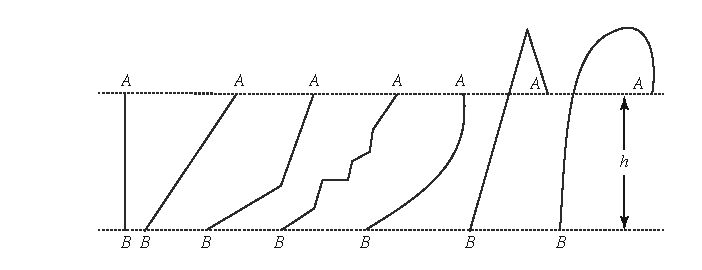
\includegraphics{images/energy-2.pdf}
\end{center}
\tagged{student}{\vspace*{3cm}}
\begin{taggedblock}{teacher}
\noindent
解析:$mgh$
\end{taggedblock}
\end{example}


\begin{example}
质量为$m$的物体在与水平方向夹角为$\theta$的恒力$F$作用下沿着摩擦系数为$\mu$的平面上前进距离为$L$,求在此过程中恒力$F$、摩擦力$f$、重力$mg$以及平面的支持力$N$所做的功。
如果初始速度为$v_0$,指向右侧,求最后该物体的速度。
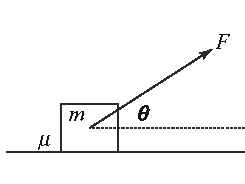
\includegraphics{images/energy-3.pdf}
\tagged{student}{\vspace*{3cm}}
\begin{taggedblock}{teacher}
\noindent
解析:$F:F\cos\theta L$   $f:fL$     $mg: 0$   $N:0$
\newline
$\frac{1}{2}mv^2=\frac{1}{2}mv_0^2+F\cos\theta L-fL$

\end{taggedblock}
\end{example}

\begin{example}
如图,质量为$m$的小球系在倔强系数为$k$、原长为$l_0$的轻弹簧一端,弹簧的另一端固定在$O$点。
开始时小球位于水平位置$A$点,此时弹簧处于原长。
当小球由位置$A$自由释放,下落到$O$点正下方位置$B$时,弹簧的伸长量为$l_0/n$,求小球到达B点时的速度。
	\begin{flushright}
		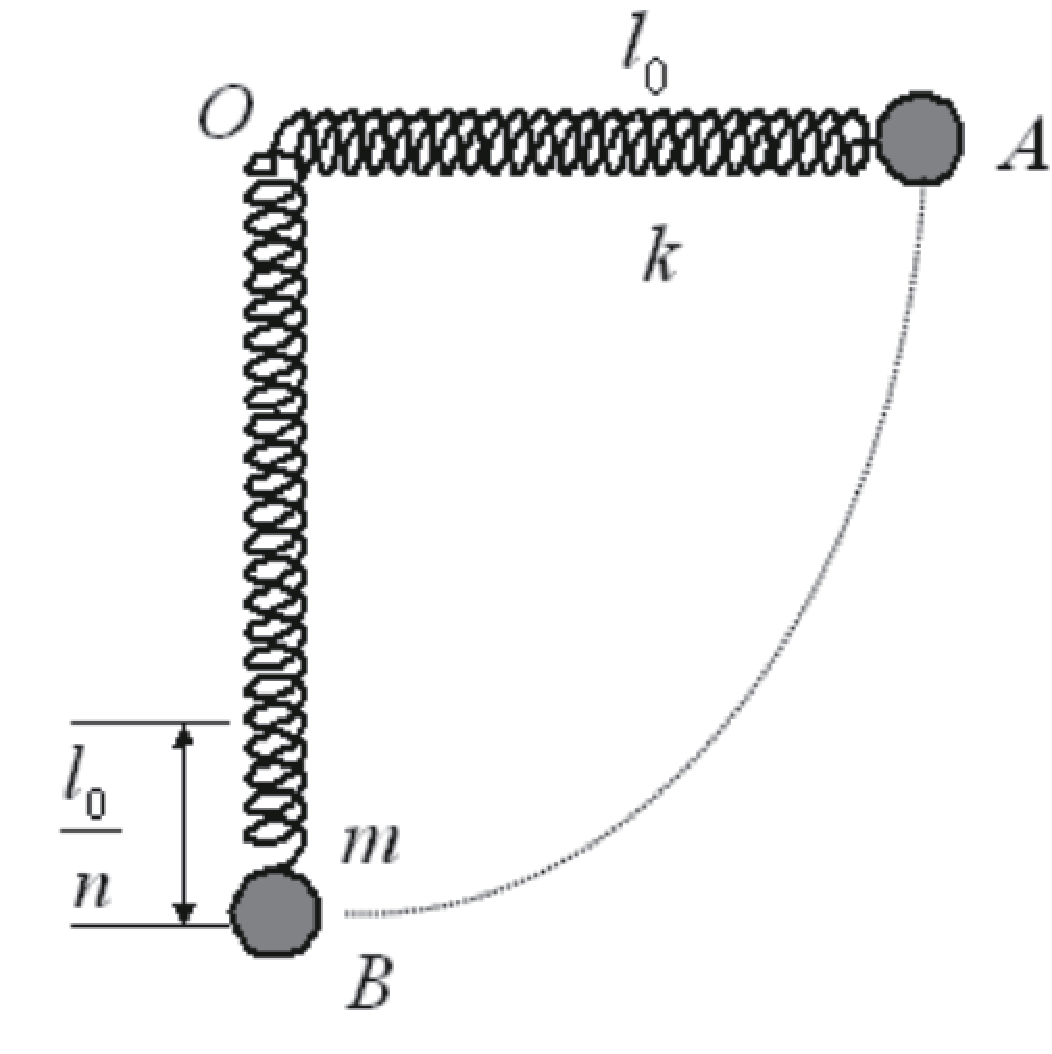
\includegraphics[width = 0.3\textwidth]{images/momentum-7.pdf} 
	\end{flushright}
\tagged{student}{\vspace*{3cm}}
\begin{taggedblock}{teacher}
\noindent
解析:$mg+\frac{mv^2}{l_0+l_0/n}=k*\frac{l_0}{n}$
\end{taggedblock}
\end{example}

\subsection{多个物体的情况}
动能定理不但可以应用到单个质点,对于由多个质点构成的力学系统同样适用,这时系统的动能被定义为内部所有质点动能的代数合。
在动量定理中我们知道,力学系统的总动量变化只由所受的外力所决定,与内力的所有性质均无关。
但在应用动能定理时内力所做的功一般来说不为零,所以在确定系统在某一物理过程前后总动能的变化时,不但要计算所有外力的功,内力做功同样不能忽略。
这样的例子不胜枚举,手枪和子弹构成的系统在子弹发射的瞬间动量毫无疑问是守恒的,但是由于火药的冲击在发射前后很明显总动能发生了明显的变化。
应用动能定理可以使我们在已知内力的功时知道始末状态各个物体的动能,反过来同样在已知始末状态后可以知道内力所做功的大小。

\begin{example}

如图所示,把弹簧的一端固定在墙上,另一端系一物体$A$,当把弹簧压缩$x_1$后,在它的右边再放一物体$B$,然后除去外力,设物体$A$和$B$均被放置在光滑的水平面上,质量分别为$m_A$和$m_B$,弹簧的劲度系数为$k$,求物体$A$移动的最大距离是多少?
	\begin{flushright}
		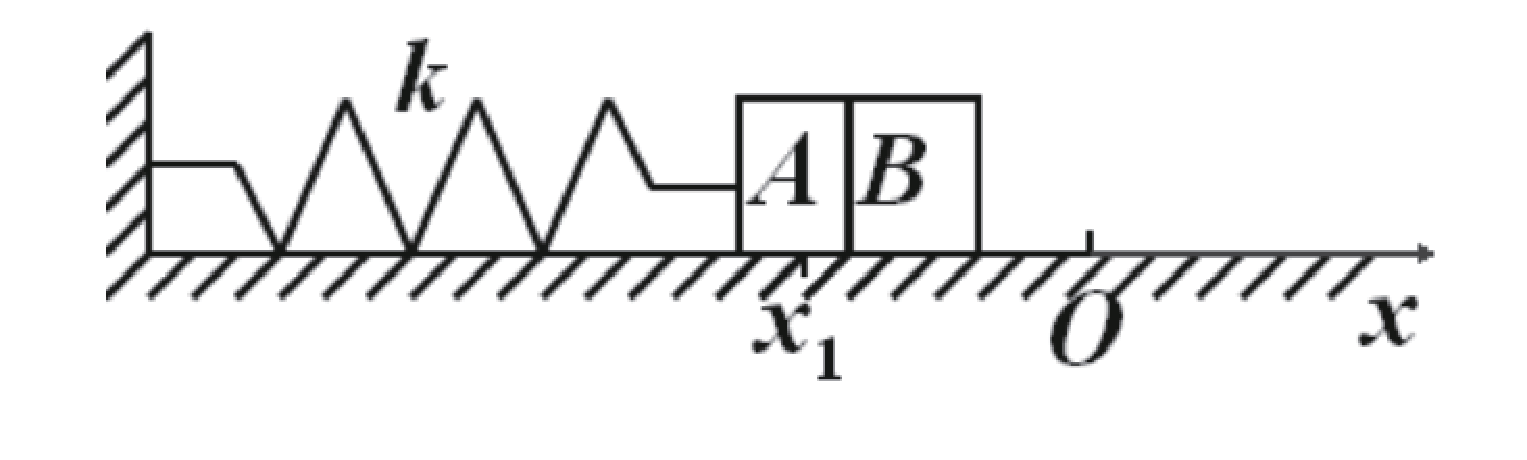
\includegraphics[width = 0.3\textwidth]{images/momentum-8.pdf} 
	\end{flushright}
\tagged{student}{\vspace*{3cm}}
\begin{taggedblock}{teacher}
\noindent
解析:$\sqrt{\frac{m_A}{m_A+m_B}}x_1+x_1$
\end{taggedblock}
\end{example}

\begin{example}
在光滑水平面上有一个足够长,质量为$M$,静止的板$B$。
设某一时刻有一个质量为$m$,速度为$v_0$的物体$A$冲入板$B$的上表面,它们之间的摩擦系数为$\mu$。
求在此后直到两者相对速度为零的过程中,两者之间的摩擦力对两个物体所做的功各是多少?
运动前后整个系统的动能变化量?
\tagged{student}{\vspace*{3cm}}
\begin{taggedblock}{teacher}
\newline
解析:对m做负功$W=\frac{mv_0^2*(M^2+2Mm)}{2(m+M)^2}$
\newline
对M做正功$W=\frac{m^2Mv_0^2}{2(m+M)^2}$
\newline
总变化量$\frac{mMv_0^2}{m+M}$
\end{taggedblock}
\end{example}

\subsection{不同参考系中的动能定理}
从运动学中我们知道描写质点的运动是需要指定参考系的,因为功的定义与力作用的距离有关而动能则依赖于运动物体的速度,这两者都与参考系的选择有关。
和所有动力学过程一样,只有在惯性(或近似)参考系中牛顿定律才能够成立,动能定理也只有在惯性参考系中才成立。

\begin{example}
在一列以速度$v_0$做均速直线运动的火车上,根据相对性原理动能定理成立。
设想火车上的一个人在光滑平面上用常力$F$拉动一个物体前进了$L$的距离,根据动能定理可以计算出该物体最终的速度。
试在相对地面静止的参考系描写同样的过程,并列出动能定理所给出的方程。
\tagged{student}{\vspace*{3cm}}
\begin{taggedblock}{teacher}
\newline
解析:略
\end{taggedblock}
\end{example}

\begin{example}
同上,但火车做加速度为$a$的匀加速过程。
以火车的参考系中分别使用动能定理能否得到正确的结果?相对地面呢?
如果想在火车的参考系中动能定理也成立,需要怎样操作呢?
\tagged{student}{\vspace*{3cm}}
\begin{taggedblock}{teacher}
\newline
解析:加入惯性力
\end{taggedblock}
\end{example}



\subsection{功与力的关系:虚功原理初步}
人与动物最大的区别就是能够使用工具,人类创造出各种各样的工作以完成各种目标。
初中已经学过了一些简单的机械:杠杆、轮轴、齿轮、滑轮等等,复杂的机械装置都是由这些基本的结构组成的。
利用机械装置可以将动力转化成所需要的形式,这其中有一个极其重要的物理原理:机械只能够传递能量,但不能创造能量。
机械一头连着动力源,可以是人力也可能是蒸气机或电动机,另一头连着输出端,用来抬起重物或者其它运动形式,但即使是最理想的,无摩擦或其它形式损耗的机械也只能够传递由动力源产生的“力”。
也就是说动力源所做的功在经过理想的机械转化后在输出端所做的功完全一样,不会变多也不会变少。

\begin{wrapfigure}{4}{50pt}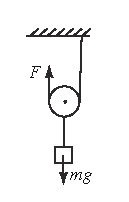
\includegraphics{images/energy-wheal.pdf}\end{wrapfigure}
右图表示一个动滑轮,下方挂上质量为$m$的重物,在力$F$作用下匀速上升。
由于滑轮的构造,当$F$的作用点上升距离为$L$时,重物只会上升一半的高度,也就是$L/2$。
由于在拉动过程中外力$F$完全用来抵抗重力,这样对于理想的滑轮,拉力的功刚好等于重力在该过程中所做的负功
\begin{equation}
F\cdot L = mg\cdot\frac{L}{2}
\end{equation}
消去所运行的距离$L$,我们得到一个拉力和重物重力的关系
\begin{equation}
F = \frac{1}{2}mg
\end{equation}
这时有意思的事情出来了,从拉力的功需要等于重力的功这样一个原理出发,我们得到了一个拉力与重力的关系,而这样的关系在过去只能通过受力分析而导出。

像这样一个能够通过做功的关系而得到作用力的关系的办法在物理上叫做\emph{虚功原理}。
利用虚功原理我们可以得到受约束的物理系统各部分之间受力的关系,在有的情况下通过静力学的办法并不容易得到。





\subsection{变力作功}
之前处理的大部分情况下都是恒力的功,其实当作用力不是恒力的时候也可以运用动能定理,只要我们能够计算在任意情况下力的功即可。
这时,在力作用下前进一段距离后该力的功\ref{eqn: 动能定理-功的微分}的表达并不是特别合适,因为它需要在每一个微小的位移上计算力与位移的夹角,这样的计算有的时候并不容易。
其实功还有另外一种描写方法。
为此建立一个任意的直角坐标系,这样外力$F$可以用它在三个坐标轴上的投影$(F_x,F_y,F_z)$来描写,与此同时在该力作用下的质点的位移同样可以用它在三个轴的投影$(\Delta x, \Delta y, \Delta z)$给出,而力在该位移下的功则可表达成

\begin{equation}
\Delta W = F_x\Delta x +F_y\Delta y+F_z\Delta z = \vec{F}\cdot\vec{\Delta r}
\end{equation}
功这样的表达方式可以帮助我们更容易地计算。
从中可以看出对于任意过程力的功可以看做三个独立方向上力的分量与位移分量的乘积的累加。

\begin{example}
假设两个物体间的相互吸引力与它们之间距离成反比,现固定其中的一个点,求另一个点由相距$r_A$到$r_B$的运动过程中上述引力所做功的大小。
\tagged{student}{\vspace*{3cm}}
\begin{taggedblock}{teacher}
\newline
解析:$F=\frac{a}{r}$   $\Delta W=F*\Delta r=\frac{a}{r}\Delta r$ 求和:$W=a*\ln\frac{r2}{r1}$
\end{taggedblock}
\end{example}


\begin{example}
假设两个物体间的相互吸引力与它们之间距离平方成反比,现固定其中的一个点,求另一个点由相距$r_A$到$r_B$的运动过程中上述引力所做功的大小。
\tagged{student}{\vspace*{3cm}}
\begin{taggedblock}{teacher}
\newline
解析:$F=\frac{a}{r^2}$   $\Delta W=F*\Delta r=\frac{a}{r}\Delta r$ 求和:$W=a*(\frac{1}{r_2}-\frac{1}{r_1})$
\end{taggedblock}
\end{example}



\section{势能、能量守恒定律}
前面学习了动能定理以及运动物体动能和外力对它做功的关系,并且能够发现不同的外力所做的功有很大的不同。
根据做功性质的不同,可以将力分为两大类。
第一种就是像重力、弹簧弹力,它们所做的功只与始末位置有关,与在力作用下物体运动轨迹无关;另一种就是像滑动摩擦力一样的各种阻力,它们做的功很明显与在阻力作用下物体所行进的距离有关,这种力比较讨厌,是工程中所极力避免的,但是又无处不在。
当一个物体在无阻力的空间中运动,或者阻力很小可以忽略不计时,它的运动具有很明显的特点,这就是本章要学习的内容--机械能守恒。

\subsection{重力作用下物体的运动}
如图\ref{fig: 从A到B沿不同光滑轨道下落的物体,将其放入某一任意的坐标系当中}所示,地球表面附近有两个给定点$A$,$B$,它们之间的高度差为$h$。
假设我们在两点之间安装多个形状不同的光滑轨道,令一个物体沿着不同的轨道从$A$点出发沿轨道下落。
\begin{figure}
\begin{center}
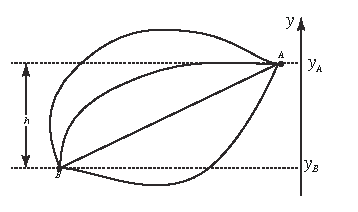
\includegraphics{images/energy-4.pdf}
\caption{从A到B沿不同光滑轨道下落的物体,将其放入某一任意的坐标系当中}
\label{fig: 从A到B沿不同光滑轨道下落的物体,将其放入某一任意的坐标系当中}
\end{center}
\end{figure}
轨道具有这样的性质,它的作用仅仅是把物体限制在轨道上,每一时刻它们之间有相互压力作用,但是压力与轨道切线永远垂直,根据功的性质,这样的压力在物体运动过程当中对运动物体的功恒为零。
这样在下落过程中仅有重力会作功,而且由于重力作功仅与始末点的高度差有关,所以在沿不同轨道下落时重力做功都相等:
\begin{equation}
W_G = mgh
\end{equation}
其中$m$为物体的质量,$h$为A、B两点间的高度差。
假设所有的物体在A点都以相同的初速率$v_A$滑向轨道,根据动能定理
\begin{equation}
mgh  = \frac{1}{2}mv_B^2-\frac{1}{2}mv_A^2
\end{equation}
很明显可以看出沿着不同轨道到达B点虽然速度的方向被轨道所限制,但是它们的动能都相同:
\begin{equation}\label{eqn: energy-B点的动能}
\frac{1}{2}mv_B^2 = \frac{1}{2}mv_A^2 + mgh
\end{equation}
它们都等于A点的动能与从A到B的过程中重力做功之和,并且与运行的轨道无关!

更进一步,建立如图所示竖直向上的坐标系,在该坐标系中A、B两点的坐标分别为$y_{A,B}$,这样我们有	
\begin{equation}
h = y_A-y_B
\end{equation}
将它代入式\ref{eqn: energy-B点的动能}可得
\begin{equation}
\frac{1}{2}mv_B^2 = \frac{1}{2}mv_A^2 + mg(y_A-y_B),
\end{equation}
进一步将其变形有
\begin{equation}\label{eqn: energy重力场中能量守恒}
\frac{1}{2}mv_B^2 + mgy_B= \frac{1}{2}mv_A^2 + mgy_A.
\end{equation}
从中可以看出,该物体在B点的动能与$mgy_B$的和与在A点的动能和$mgy_A$的和相同。
如果我们将一个物体所受的重力$mg$与它所处位置的竖直坐标$y$的乘积称为它在重力场中的\emph{势能},或者\emph{重力势能}
\begin{equation}\label{eqn: energy重力势能}
E_P(y) = mgy
\end{equation}
的话,上式可以表达为此时在A、B两点处动能与重力势能的和相同。
需要指出的是前面的推理与A、B两点所处的具体位置无关,也就是说无论它们的高度如何式\ref{eqn: energy重力场中能量守恒}均成立。
基于这个性质我们可以定义该物体的机械能为动能与重力势能的和,并且当仅存在如图\ref{fig: 从A到B沿不同光滑轨道下落的物体,将其放入某一任意的坐标系当中}所示的光滑轨道时,无论它处于何处,机械能
\begin{equation}
E = E_k+E_p = \frac{1}{2}mv^2+mgy
\end{equation}
都相同,或者说机械能为常数,该常数的大小由任意一点处动能和势能的和决定。

\begin{example}
求下列各种情况下物体所能够达到的最大高度,每种情况下都是质量为$m$,初速度为$v$
\begin{center}
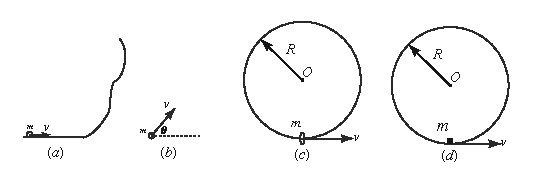
\includegraphics{images/energy-5.pdf}
\end{center}
\begin{enumerate}
\item 冲向一条无限高的弯曲的光滑轨道
\item 以与水平面夹角为$\theta$抛出
\item 套在半径为$R$的光滑圆环上运动
\item 在半径为$R$的光滑圆柱体内部运动
\end{enumerate}
\tagged{student}{\vspace*{3cm}}
\begin{taggedblock}{teacher}
\noindent
解析:$h=\frac{v^2}{2g}$
\end{taggedblock}
\end{example}

%%%%%%%%%%%%%
\begin{example}
	一个质量为$m$的质点从固定在水平面上,半径为$R$的半圆柱形表面的顶端由静止开始下落,求它脱离圆柱体的位置和圆心的连线与竖直方向的夹角$\theta$,以及它落地点与圆心的距离。
		\begin{flushright}
			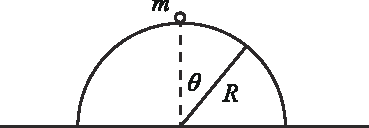
\includegraphics[width = 0.3\textwidth]{images/energy-8.pdf} 
		\end{flushright}
	\tagged{student}{\vspace*{4cm}}
	\begin{taggedblock}{teacher}
		\noindent
		解析:$mgR(1-\cos\theta)=\frac{1}{2}mv^2$   \\ $m\frac{v^2}{R}=mg\cos\theta$
	\end{taggedblock}
\end{example}
%%%%%%%%%%%%%%%%%%%%

\begin{example}

如图所示,光滑的水平面上有一个质量为$m$以初速度$v$运动的物体,冲向一个半径为$R$的光滑圆形表面,求使得它能够击中圆心$O$的初速度$v$.
\begin{flushright}
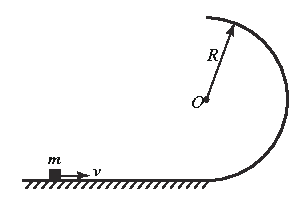
\includegraphics[width = 0.2\textwidth]{images/energy-6.pdf}
\end{flushright}
	\tagged{student}{\vspace*{4cm}}
	\begin{taggedblock}{teacher}
		\noindent
		解析:设离开轨道时物块的位置与水平面夹角为$\theta$,速度为u,则有:
		\[mgR(1+\sin\theta)=\frac{1}{2}m(v^2-u^2)\]
		\[m\frac{v^2}{R}=mg\sin\theta\]
		\[ut\sin\theta=R\cos\theta\]
		\[\frac{1}{2}gt^2-vt\cos\theta=R\sin\theta\]
		解出$v=\sqrt{2gR(1+\frac{3\sqrt{5}}{10})}$
	\end{taggedblock}
\end{example}

\subsection{保守力、势能}
从上面的例子可以看出,重力做功仅与始末位置的高度差有关,此时可以定义重力势能,当物体的运动过程中只有重力做功时它的动能与重力势能的和,并且在运动的任意时刻机械能都保持不变。

具有和重力相同性质的力称之为\emph{保守力},保守力的共同特点是
\begin{enumerate}
\item
保守力的大小和方向仅与位置有关。
重力就是一种保守力,在地表附近它的大小和方向均不变;除重力以外一端固定的弹簧弹力也是保守力的一种,它的大小与弹簧伸长量成正比,方向永远指向弹簧的固定端;除了它们以外将来会学到的万有引力,带电粒子在静电场中的电场力等也具有相同的特征。
\item 
保守力做功只与起始位置有关,与在保守力作用下物体运行的轨迹无关。
重力的情况我们已经看到了,在上一讲中我们也看到弹簧力做功也仅与始末状态的伸长量有关。
\item 一个直接推论就是沿着任意闭合路径运行的物体过程中保守力做功一定为零。
\item 对于保守力可以定义势能。
势能仅是位置的函数,与在保守力作用下物体的速度、时间等其它物理量无关。
势能由保守力的形式决定,重力势能已由式\ref{eqn: energy重力势能}给出;弹性力的势能为
\begin{equation}
E_p(x) = \frac{1}{2}kx^2
\end{equation}
其中$k$为弹性系数,$\Delta l$为弹簧的伸长量。
在反比于距离平方的吸引力作用下的势能则是

\begin{equation}
E_p(r) = -\frac{GMm}{r}
\end{equation}
其它形式的势能也可由保守力做功所确定,需要注意的是势能的定义有相对性,对于物体运动真正有意义的是始末两点的势能的差,而不是势能的大小。
这样可以将保守力作用下物体任意位置取做势能的零点,但为了方便起见我们通常会做一些约定。
\item 当已知保守力随位置的关系以后在约定了势能零点以后可以求出其它各点势能,反过来当已知势能的形式也同样可以求出力的大小和方向。
当给定各点的势能以后,通过任何一个空间中的给定点会有一个确定的曲面(或平面),该平面上各点的势能与给定点相以,这样的曲面称做\emph{等势面}。
各个点保守力的方向与等势面垂直,大小与势能变化快慢有关。
\item 如果一个物体仅受保守力作用,可以定义它的机械能为动能和势能的和。
而且在运动过程中机械能保持不变,或机械能守恒,不变的机械能可以由任意一点的机械能给出。
\end{enumerate}



%%%%%%%%%%%%%
\begin{example}
	判断以下各种力是否为保守力,如果是,试着分析它的势函数的性质
	\begin{enumerate}
		\item
		正比于时间的拉力 $f=a\cdot t$
		\item  正比于速度的阻力 $f = -\alpha v$
		\item  正比于坐标三次方的吸引力 $f = - k x^3$
		\item  随距离具有复杂形式的吸引力$f(r) = -k\frac{e^{-\alpha\cdot r} }{r^2}$ 
	\end{enumerate}
	\tagged{student}{\vspace*{4cm}}
	\begin{taggedblock}{teacher}
		\noindent
		解析:3和4是
	\end{taggedblock}
\end{example}
%%%%%%%%%%%%%%%%%%%%



\begin{example}
一个弹性系数为$k$,自然长度为$l_0$的弹簧一端固定在给定点A处,一端连着一个质量为$m$的物体,求以下各种情况弹簧的最大伸长量。
\begin{enumerate}
\item
物体在与A处于同样水平面的光滑平面运动,初始时刻弹簧位于原长,且物体具有初速度$v_1$
\item 物体在与A处于同样水平面的光滑平面运动,初始时刻弹簧压缩量为$\delta l$,初速度$v_2$,方向指向平衡位置。初速度方向背向平衡位置又如何?
\item 物体在通过A的垂线上运动,初始时刻位于原长以下$h$处,速度$v_3$竖直向上。初速度方向向下又如何?
\end{enumerate}
	\tagged{student}{\vspace*{4cm}}
	\begin{taggedblock}{teacher}
		\noindent
		解析:用能量守恒求解。最大伸长量和速度是正是反没关系。
	\end{taggedblock}
\end{example}

\section{质点系统的机械能守恒}
前面我们看到的都是单个质点在保守力作用下的机械能守恒,现在考察由多个质点构成的力学系统的机械能。
一个系统内的所有质点除了受到外力作用以外还会有相互之间满足牛顿第三定律的内力作用。
在动能定理的学习中已经发现,和动量不同,内力有可能改变系统的总动能的。
但是和一般的力一样,内力作功也有两种截然不同的情况:或者像保守力一样两个质点间的内力做功仅与两质点的相对位置有关,或者像摩擦力一样内力做功与相对运动的方式有关。
对于前一种情况虽然在内力作用下改变了系统的动能,但是实际上是动能转化为质点位置的变化,以随后的运动过程中还能够随着各个质点相对位置的改变重新释放出来而转化为各个质点的动能;而对于后一种情况,内力的作用永久地消耗了力学系统的机械能,这种消耗再也没有机会再次转化为质点的动能。

对于内力和外力都是保守力的情况,可以定义整个力学系统的总机械能为全部质点的动能、外力的势能以及系统内部质点两两之间可能的势能的和,并且我们知道系统总的机械能是守恒的。

\begin{example}
光滑水平面上有一根无质量的弹簧,劲度系数为$k$,原长为$l_0$。
它的两端分别连接质量分别为$m_1$,$m_2$的两个物体。
初始时刻两物体的速度均为零,相距$l<l_0$,求把该系统释放以后两物体之间的最大距离。
取向右为正方向,若最初时刻两物体的速度分别为$v_1$,$v_2$时,此后的运动过程中两物体最近和最远距离分别为多少。
\tagged{student}{\vspace*{4cm}}
	\begin{taggedblock}{teacher}
		\newline
		解析:最长为$2l_0-l$,若有速度,最长与最短为$l_0\pm\sqrt{\frac{m_1m_2g}{(m_1+m_2)k}(v_2-v_1)^2+(l_0-l)^2}$
	\end{taggedblock}
\end{example}


\begin{example}
两个质量分别为$m_1$,$m_2$的两个物体用原长为$l_0$,劲度系数为$k$的轻弹簧连接,
初始时刻A放在B的上方且均为静止,将弹簧压缩至$l<l_0$,求将系统释放以后B能够离开地面的条件。
	\tagged{student}{\vspace*{4cm}}
	\begin{taggedblock}{teacher}
		\newline
		解析:离开地面条件为$l_0-l\geq\frac{(2m_1+m_2)g}{k}$
	\end{taggedblock}
\end{example}

\begin{example}
在光滑的平面上两个球A,B,质量分别为$m_A$、$m_B$。
开始时刻B球静止,A球以速度$v_0$撞向B。
如果碰撞之后两球运动速度均与A的初速度方向相同,且碰撞过程极短,无机械能损失,求碰后两个物体的速度分别为多少?
	\tagged{student}{\vspace*{4cm}}
	\begin{taggedblock}{teacher}
		\newline
		解析:设碰后A的速度为$v_1$,B的速度为$v_2$,
		\[m_Av_1+m_Bv_2=m_Av_0\]
		\[\frac{1}{2}m_Av_1^2+\frac{1}{2}m_Bv_2^2=\frac{1}{2}m_Av_0^2\]
		解出\[v_1=\frac{m_A-m_B}{m_A+m_B}v_0\]\[v_2=\frac{2m_A}{m_A+m_B}v_0\]
	\end{taggedblock}
\end{example}


\begin{example}
光滑平面上有两个质量相同的球A、B。
A球以某一初速度$v_0$撞向B,求证无论A球以何种方式弹开,B球的速度方向永远与A球弹开的方向垂直,假设碰撞时间极短,无机械能损失。
\tagged{student}{\vspace*{4cm}}
	\begin{taggedblock}{teacher}
		\newline
		解析:略
	\end{taggedblock}
\end{example}





\subsection{机械能的损失:摩擦}
当一个物体所受的力中包含有非保守力时,机械能将不再守恒,熟知的滑动摩擦力就是这样的一种力,它会使得机械能永久消失。
对于单个质点,将它所受的外力分为保守力和非保守力,那么在一个由A点到B点的运动过程前后根据动能定理
\begin{equation}
\frac{1}{2}mv_B^2-\frac{1}{2}mv_A^2 = W_C+W_{NC}
\end{equation}
其中$W_C$和$W_{NC}$分别表示保守力和非保守力的功,根据保守力的性质可知
\begin{equation}
W_C =  -E_p(B)+E_p(A)
\end{equation}
其中$E_p(B)$、$E_p(A)$分别代表A、B两点的势能。
这样将上式整理可得
\begin{equation}\label{eqn: energy非保守力的能量定理}
W_{NC} = \left(\frac{1}{2}mv_B^2+E_p(B)\right)-\left(\frac{1}{2}mv_A^2+E_p(A)\right) = E(B)-E(A)
\end{equation}
也就是说,非保守力的功等于运动前后总机械能的变化量。
摩擦力一般情况下会做负功,使得总的机械能减小,当然还有其它形式的非保守力有可能增加物体的机械能。

\begin{example}
在一个沿着粗糙斜面下滑的物体验证式\ref{eqn: energy非保守力的能量定理}。
一个由静止出发沿着摩擦系数为$\mu$,倾角为$\theta$的粗糙斜面下滑,求当滑下距离为$L$时它的速度。
	\tagged{student}{\vspace*{4cm}}
	\begin{taggedblock}{teacher}
		\newline
		解析:略
	\end{taggedblock}
\end{example}


\begin{example}

如图所示,一轻弹簧,一端固定在墙上,另一端连一小物块。
小物块放在摩擦系数为$\mu$的水平面上,弹簧处在自然状态,小物块位于O处。
现用手将小物块向右移到a处,然后从静止释放小物块,发现小物块开始向左移动。
\begin{flushright}
\includegraphics{images/energy-7.pdf}
\end{flushright}

\begin{description}
\item[ A]小物块可能停在O点
\item[B] 小物块停止以后所受的摩擦力必不为0
\item[C] 小物块无论停在O点左边还是右边,停前所受的摩擦力的方向和停止后所受摩擦力的方向两者既可能相同也可能相反
\item[D] 小物块在通过O点后向右运动直到最远处的过程中,速度的大小总是减小;小物块在由右边最远处回到O点的过程中,速度大小总是增大。
\end{description}
	\tagged{student}{\vspace*{4cm}}
	\begin{taggedblock}{teacher}
		\noindent
		解析:AC
	\end{taggedblock}
\end{example}
对于更复杂过程中的机械能的变化也可以通过类似的物理分析得出结论。



\section{能量的转化与守恒定律}
由摩擦力或其它非保守力作用下的物体虽然会损失或增加机械能。
从更大的视角看待这个问题时我们会发现,实际上机械能并不是所有的能量,仅仅是更普遍意义下能量的一种表现形式。
由于非保守力做功而损失掉的机械能并没有从自然界消失,而是转化成了其它的形式。
无数的经验告诉我们,自然界中的能量并不会增加,也不会减少,而是在不同物体,不同运动形式之间不段地转化。
物理学研究的对象可以没有质量、可以没有速度、甚至连确定的位置都没有,但是它们无一例外地具有能量,一个没有能量或其能量无法与转化为我们可感知形式的对象根本无法和我们发生相互作用,被我们所感知和研究。

能量存在的形式有很多,在力学中我们已经见过了由于物体运动而具有的动能,由于所处位置不同而具有的势能,除此以外还有很多其它形式。
从某种意义上讲物理就是一个研究能量的不同存在形式以及在这些不同存在形式之间相如何相互转化的学科。
在认识能量的过程中人们走过了很多的弯路,甚至一些非常具有影响力的科学家在面对新的实验现象时也曾经怀疑过自然界的能量是否真的守恒,但事实一次次地证明,能量的守恒定律是自然界运行的最基本的定律,在任何时候,对于任何物理过程,无论简单或复杂、无论能否被直接观测,都无一例外是守恒的。














